% In Lab 3, we looked at simulating the Von K´arm´an Vortex Street in the wake of a 2D
% circular cylinder. In this assignment, we build on our finding in Lab 3 to simulate the
% unsteady vortex shedding phenomenon due to a laminar flow of air at 25◦C over an infinitely
% span circular cylinder. The cylinder spans across the entire computational domain as shown
% by the problem schematics in Figure 1, where the cylinder diameter (D) is 10 mm, the free
% stream velocity is U∞ = 0.2 m/s in the streamwise (x−) direction, uniformly.
% Figure 1: Schematics of the computational domain for the flow over a circular cylinder.
% 1
% The problem looks at the unsteady wake of a two-dimensional cylinder. The objectives of
% this lab assignment are:
% (I) Setting up an unsteady simulation in ANSYS Fluent using ANSYS Workbench,
% (II) Effect of timestep on performance of the solvers.
% PART I. Problem Setup
% In this lab, we will build on our findings from Lab 3, where we examined the mesh- independence for a 2D circular cylinder. Here, we use the same boundary conditions and general
% setup, as shown in Figure 1.
% Considering the setup in Figure 1, complete the following tasks:
% Task 1.1. Calculate the problem Reynolds number (Re = U∞D/ν) and confirm that the
% flow is laminar.
% Task 1.2. Open ANSYS Workbench and define a new project based on ANSYS Fluent.
% Download “grid3-mesh” from eClass. Import the mesh into the Fluent project and proceed
% with the “Setup”.
% Task 1.3. Change analysis type to Transient under “General”. Calculate the minimum
% timestep for unsteady simulations based on the minimum element size of “Grid 3”. You
% need to use the Courant (CFL) number for this estimation. Set the simulation timestep
% according to your calculations, while keeping the estimated CFL number below 0.8.
% Task 1.4. Calculate the Through-Time (Tthr) for this setup, which is defined as the time it
% takes air to travel from the inlet to the outlet without any disturbance. Knowing the inlet
% velocity (U∞) and length of the computational domain (Lcv),
% Tthr = Lcv/U∞ (1)
% The total time of the simulation should be 10 Tthr.
% Task 1.5. In ANSYS Fluent, assign the relevant boundary conditions to the domain as it
% has been described in Figure 1. The outlet boundary condition is “Outlet” with a relative
% “Gauge Pressure” of 0 atm.
% Task 1.6. Assign the “Coupled” scheme as the pressure-velocity coupling method. Spatial
% discretizations for pressure and momentum should be second order accurate. You can change
% the solver method under “Solution” in ANSYS Fluent.
% Task 1.7. Under “Monitors”, set a “Report Plot” for measuring Pressure, Velocity Components at P1 = (D, 0, 0). Note that these parameters needs to be defined in “Report
% Definitions”. Similarly, define drag and lift forces and plot them as a function of simulation
% time.
% 2
% Task 1.8. Autosave should be configured to save at least twice per simulation second. It is
% located under “Calculation Activities”.
% Task 1.9. Ensure to enable “Data Sampling for Time Statistics” located within the “Run
% Calculation” section. This feature facilitates the collection of time-averaged quantities, such
% as mean velocity or pressure.
% PART II. Reference Simulation
% Since our computational power is limited, we will provide a solution for the reference simulation. To this end, download Lab 4 folder from eClass and proceed with the “Solution”.
% Complete the simulation of laminar unsteady flow of air over a 2D circular cylinder using
% “Grid 3” and a timestep of δt = 0.0025 s. The provided cases contains the solution until
% t = 5.5 s. Run the the cases for 0.5 s more without performing any initialization.
% Once the simulation is complete, proceed to ANSYS CFD-Post for post-processing of the
% data. Obtain or calculate the following:
% (I) Calculate the Mean Drag and Lift Coefficient for the cylinder.
% (II) Plot the monitor point data (Pressure and Velocity Components) at P1 as a function of
% time. What is the period of vortex shedding from these plots? What is the normalized
% frequency of vortex shedding or the Strauhal number (St)?
% (III) Create a contour plot of pressure (p) on the xy−plane. Adjust the values of maximum
% and minimum pressure so that the vortex shedding is distinguishable from the flow.
% (IV) Create a contour plot of spanwise vorticity (ωz) on the xy−plane. Adjust the values of
% maximum and minimum vorticity so that the vortex shedding is distinguishable from
% the flow.
% (V) Draw the plot of mean streamwise (x−direction) velocity (u) along the wake centerline
% and calculate the normalized value of Lr, which is the mean recirculation length.
% (VI) Create a contour plot of mean pressure (p) on the xy−plane. Adjust the values of
% maximum and minimum pressure so that the recirculation vortex is distinguishable
% from the flow.
% PART III. Timestep Sensitivity Analysis
% Based on the setup from PART I, repeat the simulation after changing the timestep value
% to δt = 0.025 s and δt = 0.25 s, which should be labeled as “Grid 3-2” and “Grid 3-3”,
% respectively.
% 3
% Task 3.1. Once the simulations are complete, proceed to ANSYS CFD-Post for postprocessing of the data. Re-generate the plots and calculate the parameters as listed in
% PART II.
% Task 3.2. Create a table that shows the main wake parameters (Mean Recirculation Length,
% Mean Drag Cofficient, Mean Lift Cofficient, and St) you calculated for “Grid 3”, “Grid 3-2”
% and “Grid 3-3”. Include their percentage change with respect to those of “Grid 2”. Also,
% compare the contour plots of pressure and mean pressure for the three cases.
% Task 3.3. Comment on the dfferences between the three temporal grids. Which case should
% be appropriate for wake analysis? Why?

\section{Part I. Problem Setup}
\subsection{Task 1.1}
\textit{Calculate the problem Reynolds number (Re = $U_\infty D/\nu$) and confirm that the flow is laminar.}

The working fluid is air. The properties of air at 25°C and 1 atm are taken from a textbook \cite{Cengel2017-jf}.
\begin{align*}
    \rho &= 1.184 \text{ kg/m}^3 \\
    \nu &= 1.562 \times 10^{-5} \text{ m}^2/\text{s}
\end{align*}

The Reynolds number is calculated as
\begin{align*}
    \text{Re} &= \frac{U_\infty D}{\nu} \\
    &= \frac{0.20  \times 0.01}{1.562 \times 10^{-5}} \\
    &= \boxed{128.04}
\end{align*}
This is less than the critical Reynolds number of 2000, so the flow is laminar.

\subsection{Task 1.3}
\textit{Calculate the minimum timestep for unsteady simulations based on the minimum element size of “Grid 3”. You need to use the Courant (CFL) number for this estimation. Set the simulation timestep according to your calculations, while keeping the estimated CFL number below 0.8.}

First we desire CFL to be 
\begin{align*}
    \text{CFL} &= \frac{U_\infty \Delta t}{\Delta x} < 0.8
\end{align*}
For Grid 3, the element size was selected such that $\Delta x = D/15 = 0.667$ mm. The minimum timestep is then
\begin{align*}
    \Delta t &= \frac{0.8 \Delta x}{U_\infty} \\
    &= \frac{0.8 \times 0.667 \times 10^{-3}}{0.20} \\
    &= 2.67 \times 10^{-3} \text{ s} \\
    &\approx \boxed{0.0025} \text{ s}
\end{align*}

\subsection{Task 1.4}
\textit{Calculate the Through-Time ($T_thr$) for this setup, which is defined as the time it takes air to travel from the inlet to the outlet without any disturbance. Knowing the inlet velocity ($U_\infty$) and length of the computational domain ($L_{cv}$),}
\begin{align*}
    T_{thr} &= \frac{L_{cv}}{U_\infty}
\end{align*}
\textit{The total time of the simulation should be 10 $T_{thr}$.}

\begin{align*}
    T_{thr} &= \frac{L_{cv}}{U_\infty} \\
    &= \frac{20D}{U_\infty} \\
    &= \frac{20 \times 0.01}{0.20} \\
    &= \boxed{1} \text{ s}
\end{align*}
The total time of the simulation should be 10 $T_{thr}$,
\begin{align*}
    T_{\text{total}} &= 10 T_{thr} \\
    &= 10 \times 1 \\
    &= \boxed{10} \text{ s}
\end{align*}
The number of iterations is then,
\begin{align*}
    \text{Iterations} &= \frac{T_{\text{total}}}{\Delta t} \\
    &= \frac{10}{0.0025} \\
    &= \boxed{4000}
\end{align*}

\subsection{Task 1.9}
\begin{figure}[H]
    \centering
    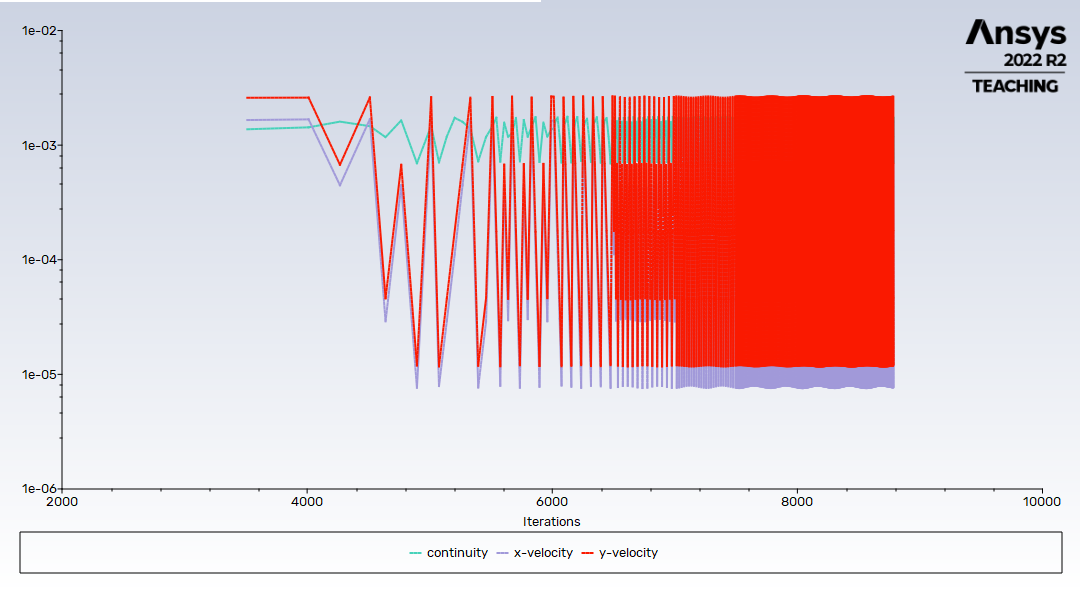
\includegraphics[width=0.8\textwidth]{Questions/Figures/residuals plot grid 3.png}
    \caption{Residuals for Grid 3}
\end{figure}

\section{Part II. Reference Simulation}

% \subsection{Summary for Grids 1, 2, 3, and 4}
% \begin{table}[H]
%     \centering
%     \caption{Summary of Results for Grids 1, 2, 3, and 4 (for ease of marking)}
%     \begin{tabular}{ccccc}
%         \toprule
%         Grid & $F_D$ & $C_d$ & $L_r$ \\ 
%         & (N) & & \\
%         \midrule
%         1 & $4.08667 \times 10^{-7}$ & $1.2 \times 10^{-4}$ & 32.5 \\
%         2 & $3.97047 \times 10^{-7}$ & $1.16 \times 10^{-4}$ & 43.0 \\
%         3 & $3.97047 \times 10^{-7}$ & $1.16 \times 10^{-4}$ & 44.0 \\
%         4 & $3.92433 \times 10^{-7}$ & $1.15 \times 10^{-4}$ & 44.0 \\
%         \bottomrule
%     \end{tabular}
% \end{table}

\subsection{(I)}
\textit{Calculate the Mean Drag and Lift Coefficient for the cylinder.}
Drag and lift plots are shown in Figures \ref{fig:drag force plot grid 3} and \ref{fig:lift force plot grid 3}. The mean drag force is
\begin{figure}[H]
    \centering
    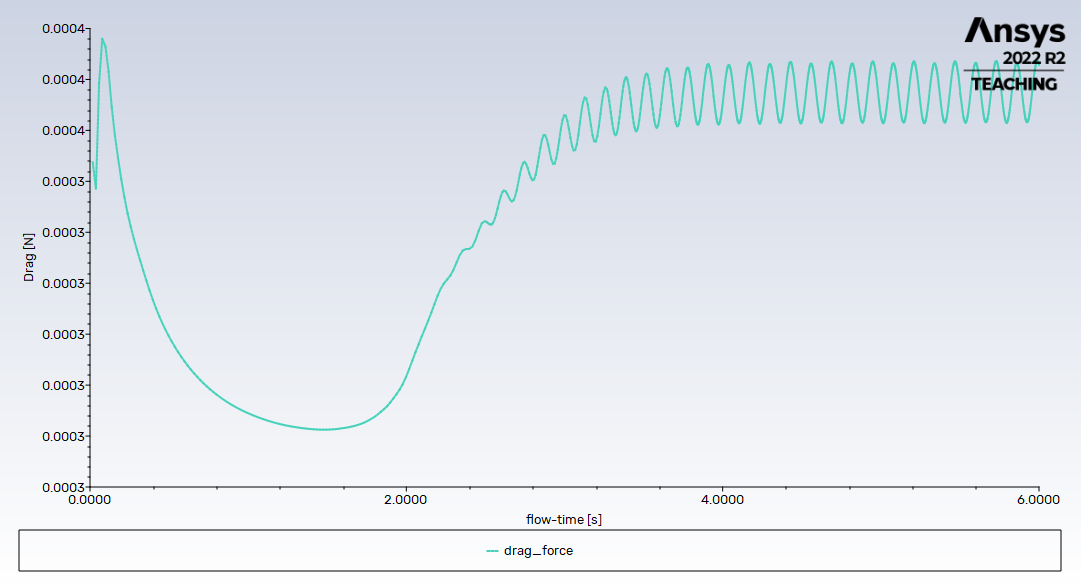
\includegraphics[width=0.8\textwidth]{Questions/Figures/drag force plot grid 3.png}
    \caption{Drag force over time for Grid 3}
    \label{fig:drag force plot grid 3}
\end{figure}
\begin{figure}[H]
    \centering
    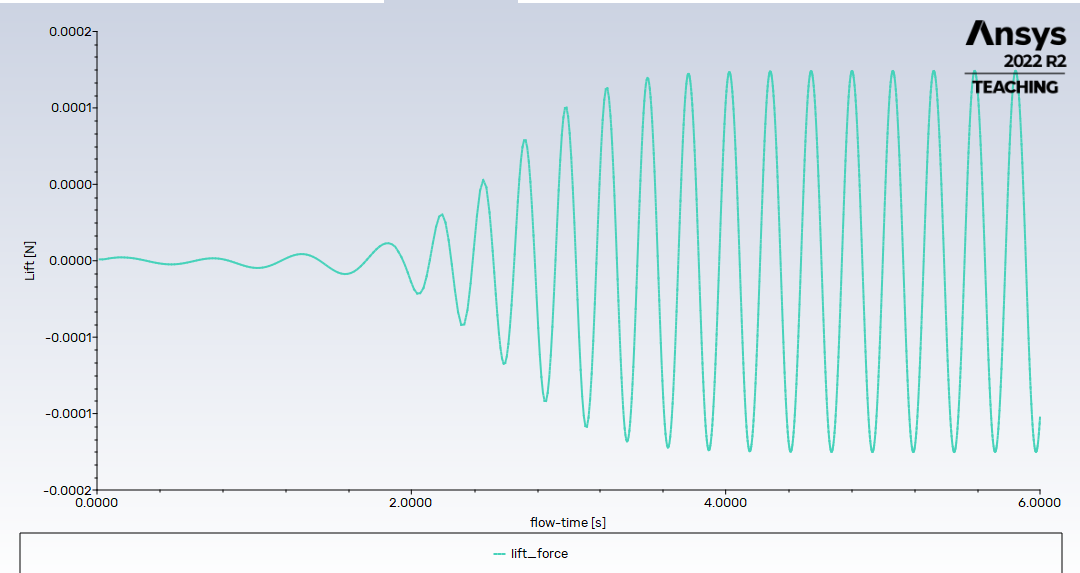
\includegraphics[width=0.8\textwidth]{Questions/Figures/lift force plot grid 3.png}
    \caption{Lift force over time for Grid 3}
    \label{fig:lift force plot grid 3}
\end{figure}
The mean drag force can be found by averaging the peak-to-trough values of the force over one period of vortex shedding in the quasi steady state region. This value was found to be
\begin{align*}
    F_D &= \frac{F_{D_{\text{max}}} + F_{D_{\text{min}}}}{2} \\
    &= \frac{3.64 \times 10^{-4} + 3.52 \times 10^{-4}}{2} \\
    &= \boxed{3.58 \times 10^{-4} \text{ N}}
\end{align*}
Similarly, the mean lift force was found to be
\begin{align*}
    F_L &= \frac{F_{L_{\text{max}}} + F_{L_{\text{min}}}}{2} \\
    &= \frac{1.24 \times 10^{-4} - 1.25 \times 10^{-4}}{2} \\
    &= \boxed{-4.40 \times 10^{-7} \text{ N}}
\end{align*}
The mean drag coefficient is then
\begin{align*}
    C_d &= \frac{F_D}{0.5\rho U_\infty^2 D} \\
    &= \frac{3.58 \times 10^{-4}}{0.5 \times 1.184 \times 0.20^2 \times 0.01} \\
    &= \boxed{1.512}
\end{align*}
The mean lift coefficient is
\begin{align*}
    C_l &= \frac{F_L}{0.5\rho U_\infty^2 D} \\
    &= \frac{-4.40 \times 10^{-7}}{0.5 \times 1.184 \times 0.20^2 \times 0.01} \\
    &= \boxed{-0.00186}
\end{align*}

\subsection{(II)}
\textit{Plot the monitor point data (Pressure and Velocity Components) at P1 as a function of time. What is the period of vortex shedding from these plots? What is the normalized frequency of vortex shedding or the Strouhal number (St)?}
\begin{figure}[H]
    \centering
    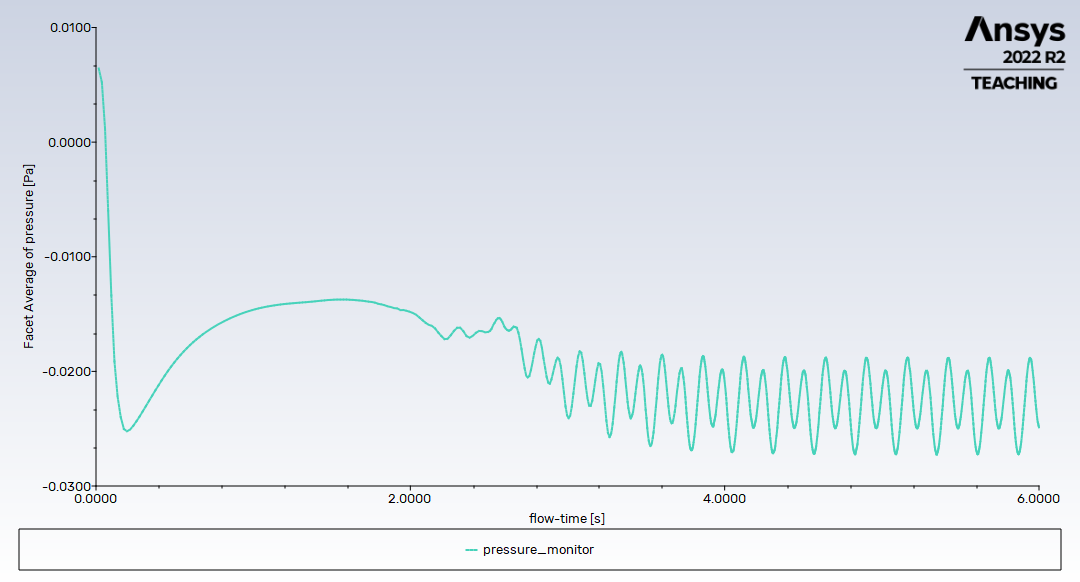
\includegraphics[width=0.8\textwidth]{Questions/Figures/pressure plot grid 3.png}
    \caption{Pressure at P1 over time for Grid 3}
\end{figure}
\begin{figure}[H]
    \centering
    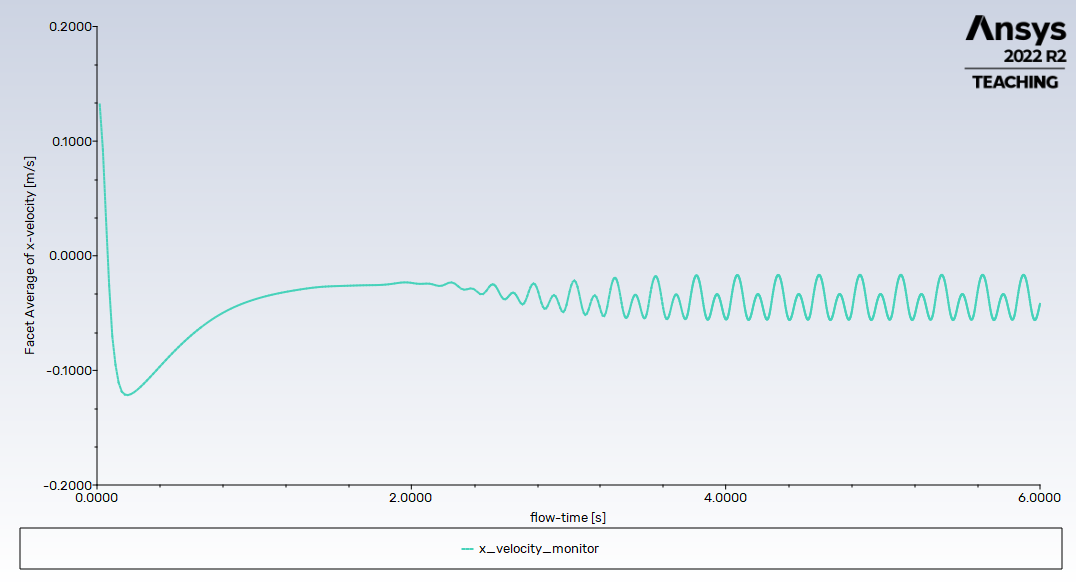
\includegraphics[width=0.8\textwidth]{Questions/Figures/x-velocity plot grid 3.png}
    \caption{Streamwise velocity at P1 over time for Grid 3}
\end{figure}
\begin{figure}[H]
    \centering
    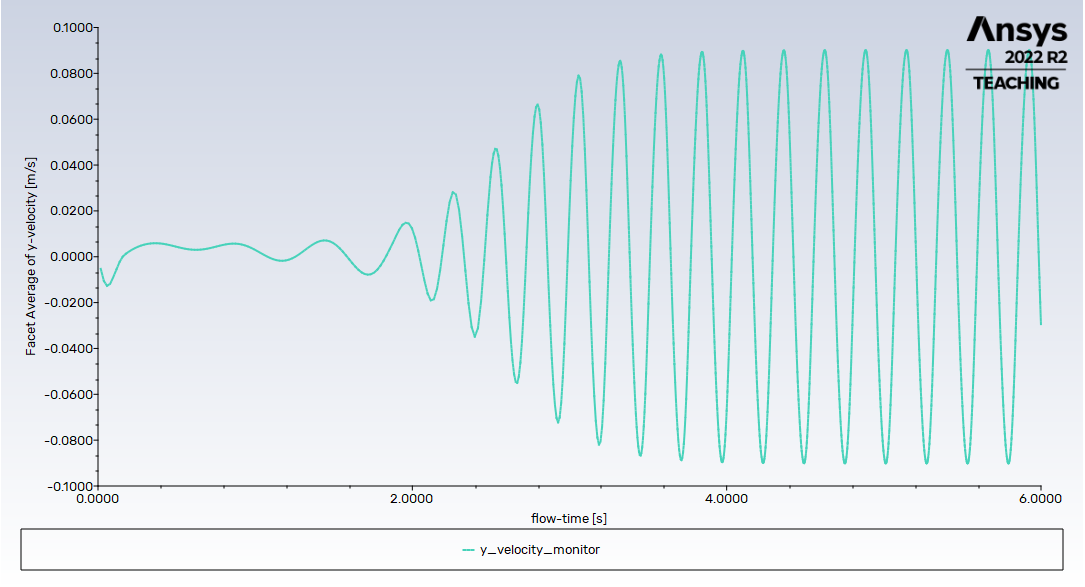
\includegraphics[width=0.8\textwidth]{Questions/Figures/y-velocity plot grid 3.png}
    \caption{Spanwise velocity at P1 over time for Grid 3}
\end{figure}
The period of vortex shedding is obtained from analyzing the y-plot in the quasi steady state region $t > 3.5$ s. The period is approximately
\begin{align*}
    \tau &= 2(t_{\text{peak}} - t_{\text{trough}})
    &= 2(5.975 - 5.845) \\
    &= \boxed{0.265} \text{ s}
\end{align*}
The Strouhal number is then
\begin{align*}
    \text{St} &= \frac{fD}{U_\infty} \\
    &= \frac{1/0.265 \times 0.01}{0.20} \\ 
    &= \boxed{0.1887}
\end{align*}

\subsection{(III)}
\textit{Create a contour plot of pressure (p) on the xy-plane. Adjust the values of maximum and minimum pressure so that the vortex shedding is distinguishable from the flow.}
\begin{figure}[H]
    \centering
    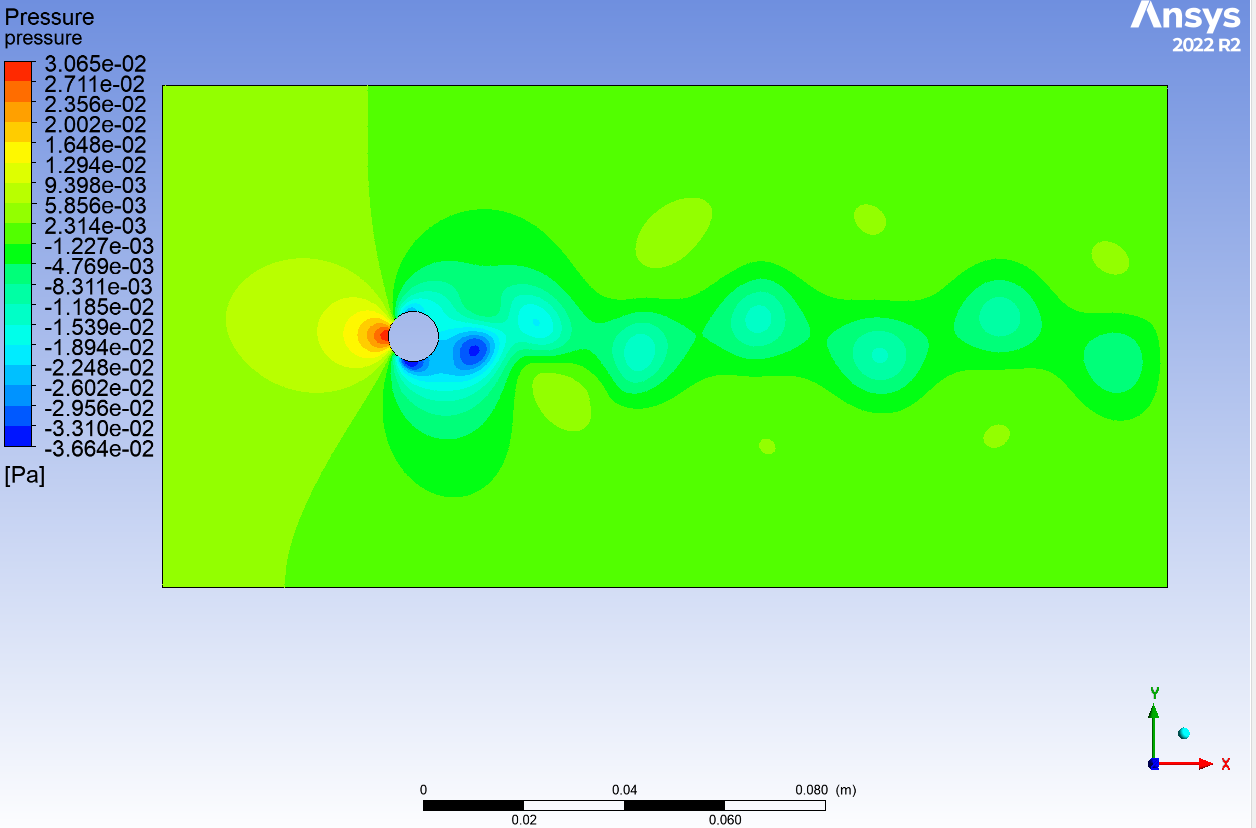
\includegraphics[width=0.8\textwidth]{Questions/Figures/pressure contour grid 3.png}
    \caption{Pressure Contour for Grid 3}
    \label{fig:pressure contour grid 3}
\end{figure}

\subsection{(IV)}
\textit{Create a contour plot of spanwise vorticity ($\omega_z$) on the xy-plane. Adjust the values of maximum and minimum vorticity so that the vortex shedding is distinguishable from the flow.}
\begin{figure}[H]
    \centering
    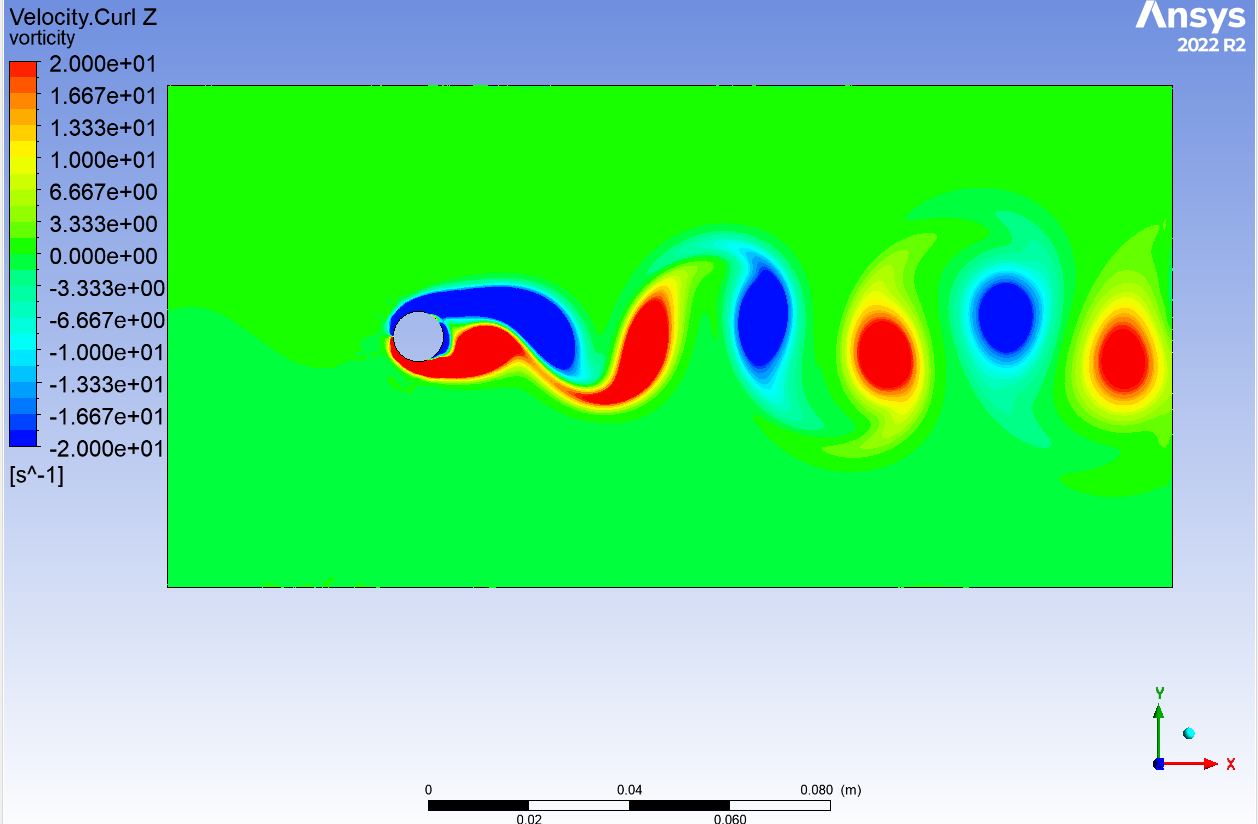
\includegraphics[width=0.8\textwidth]{Questions/Figures/vorticity contour grid 3.png}
    \caption{Vorticity Contour for Grid 3}
\end{figure}

\subsection{(V)}
\textit{Draw the plot of mean streamwise ($x$-direction) velocity ($u$) along the wake centerline and calculate the normalized value of $L_r$, which is the mean recirculation length.}

\begin{figure}[H]
    \centering
    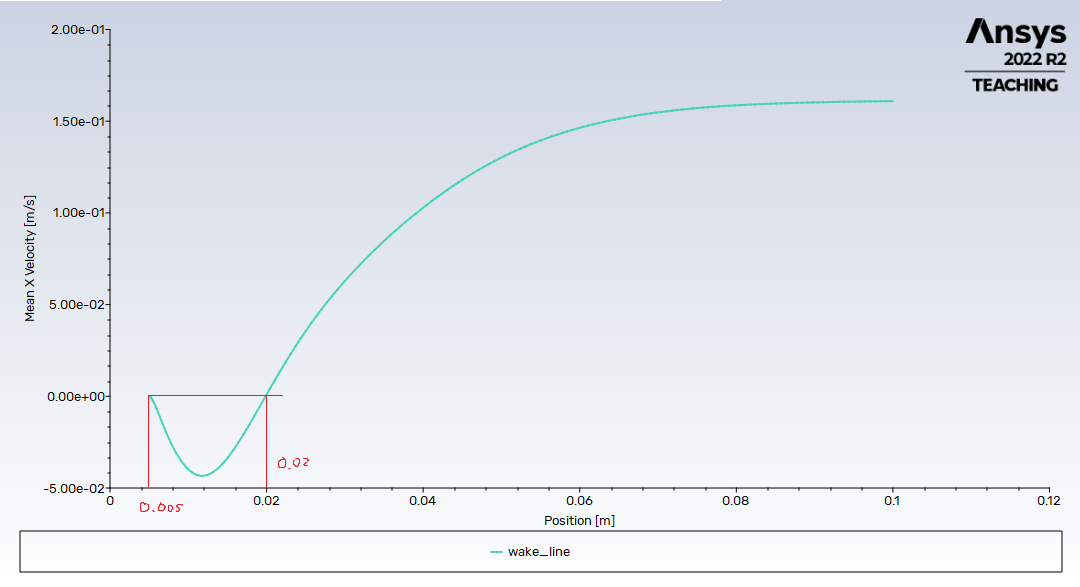
\includegraphics[width=0.8\textwidth]{Questions/Figures/mean x velocity along wake center line grid 3.png}
    \caption{Mean Streamwise Velocity for Grid 3}
\end{figure}
From the plot, the recirculation length is approximately
\begin{align*}
    \hat{L}_r &= \frac{\Delta x}{D} \\
    &= \frac{0.02 - 0.005}{0.01} \\
    &= \boxed{1.5}
\end{align*}

\subsection{(VI)}
\textit{Create a contour plot of mean pressure ($p$) on the xy-plane. Adjust the values of maximum and minimum pressure so that the recirculation vortex is distinguishable from the flow.}
\begin{figure}[H]
    \centering
    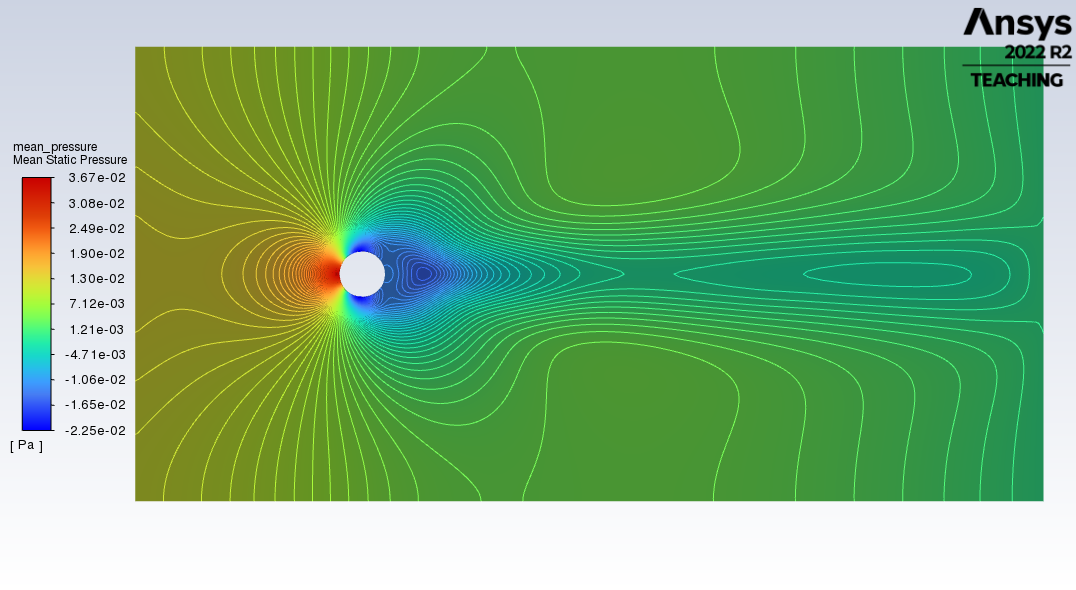
\includegraphics[width=0.8\textwidth]{Questions/Figures/mean pressure velocity contour grid 3.png}
    \caption{Mean Pressure Contour for Grid 3}
    \label{fig:mean pressure velocity contour grid 3}
\end{figure}

\section{Part III. Timestep Sensitivity Analysis}
\textit{Based on the setup from PART I, repeat the simulation after changing the timestep value to $\delta t = 0.025$ s and $\delta t = 0.25$ s, which should be labeled as “Grid 3-2” and “Grid 3-3”, respectively.}
\subsection{Task 3.1}
\textit{Once the simulations are complete, proceed to ANSYS CFD-Post for post-processing of the data. Re-generate the plots and calculate the parameters as listed in PART II.}
\subsubsection{Grid 3-2}
The number of iterations has been updated to
\begin{align*}
    \text{Iterations} &= \frac{T_{\text{total}}}{\Delta t} \\
    &= \frac{10}{0.025} \\
    &= \boxed{400}
\end{align*}

\begin{figure}[H]
    \centering
    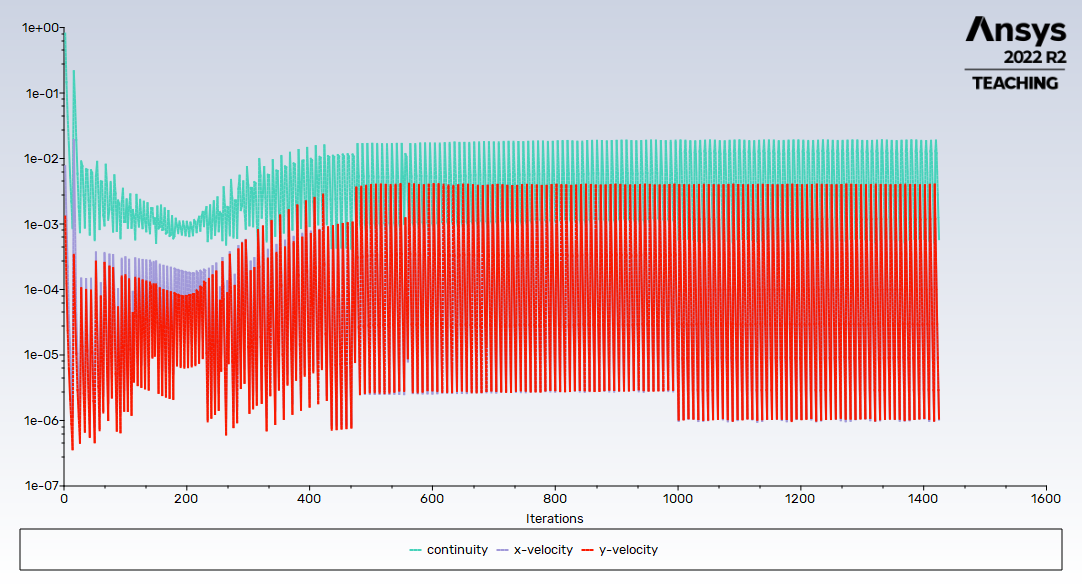
\includegraphics[width=0.8\textwidth]{Questions/Figures/residuals plot grid 3 2.png}
    \caption{Residuals for Grid 3-2}
\end{figure}

The mean and drag plots are shown in Figures \ref{fig:drag force plot grid 3 2} and \ref{fig:lift force plot grid 3 2}.
\begin{figure}[H]
    \centering
    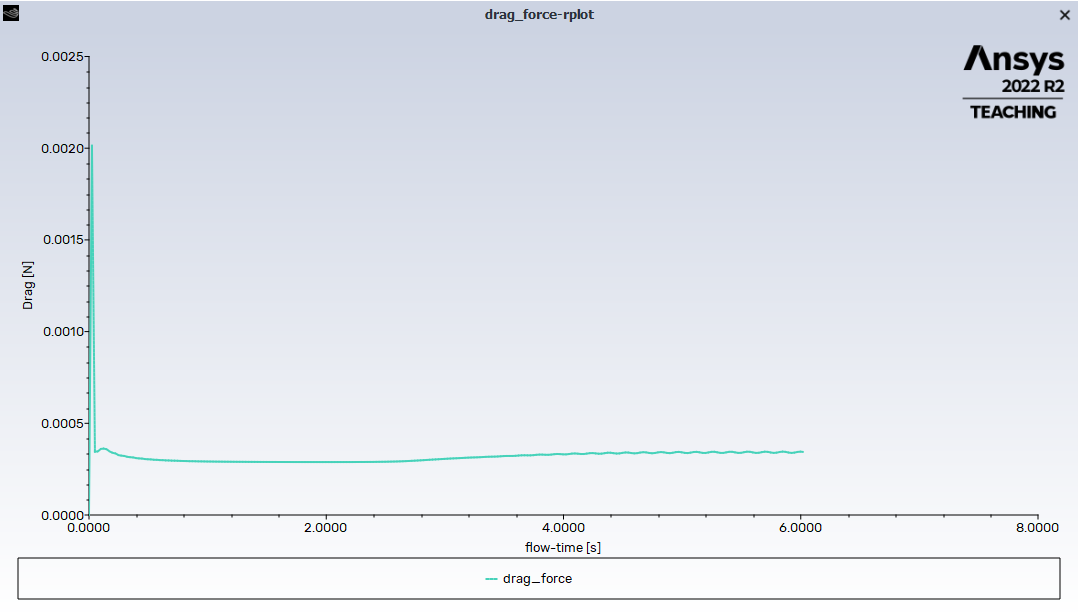
\includegraphics[width=0.8\textwidth]{Questions/Figures/drag force plot grid 3 2.png}
    \caption{Drag force over time for Grid 3-2}
    \label{fig:drag force plot grid 3 2}
\end{figure}
\begin{figure}[H]
    \centering
    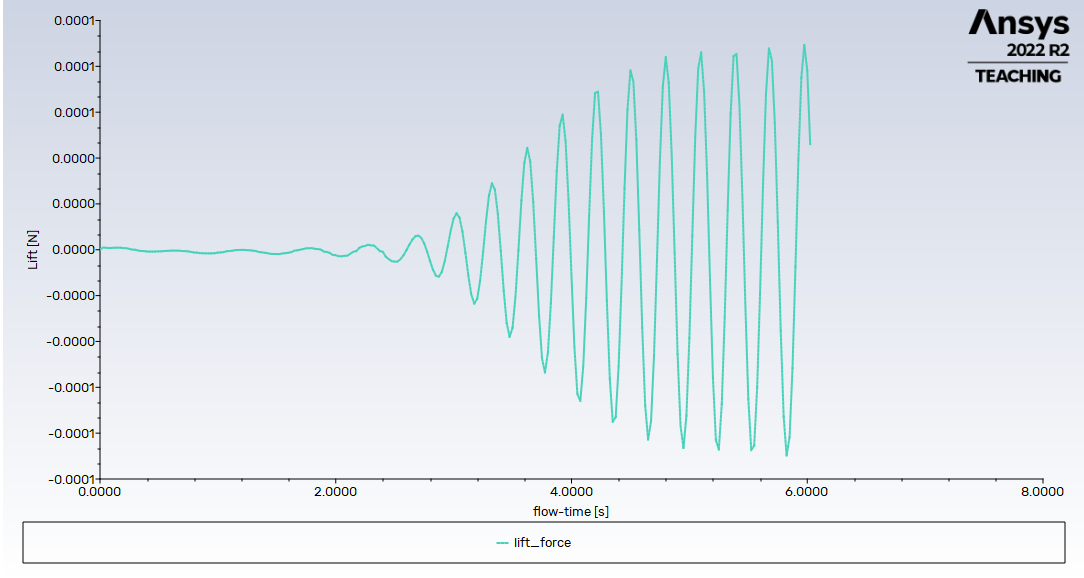
\includegraphics[width=0.8\textwidth]{Questions/Figures/lift force plot grid 3 2.png}
    \caption{Lift force over time for Grid 3-2}
    \label{fig:lift force plot grid 3 2}
\end{figure}
The mean drag force is
\begin{align*}
    F_D &= \frac{F_{D_{\text{max}}} + F_{D_{\text{min}}}}{2} \\
    &= \frac{3.46 \times 10^{-4} + 3.38 \times 10^{-4}}{2} \\
    &= \boxed{3.42 \times 10^{-4} \text{ N}}
\end{align*}
The mean lift force is
\begin{align*}
    F_L &= \frac{F_{L_{\text{max}}} + F_{L_{\text{min}}}}{2} \\
    &= \frac{8.92 \times 10^{-5} - 8.98 \times 10^{-5}}{2} \\
    &= \boxed{-2.84 \times 10^{-7} \text{ N}}
\end{align*}
Then, the mean drag coefficient is
\begin{align*}
    C_d &= \frac{F_D}{0.5\rho U_\infty^2 D} \\
    &= \frac{3.42 \times 10^{-4}}{0.5 \times 1.184 \times 0.20^2 \times 0.01} \\
    &= \boxed{1.444}
\end{align*}
The mean lift coefficient is
\begin{align*}
    C_l &= \frac{F_L}{0.5\rho U_\infty^2 D} \\
    &= \frac{-2.84 \times 10^{-7}}{0.5 \times 1.184 \times 0.20^2 \times 0.01} \\
    &= \boxed{-0.00112}
\end{align*}

The pressure and velocity plots are shown in Figures \ref{fig:pressure plot grid 3 2}, \ref{fig:x-velocity plot grid 3 2}, and \ref{fig:y-velocity plot grid 3 2}.
\begin{figure}[H]
    \centering
    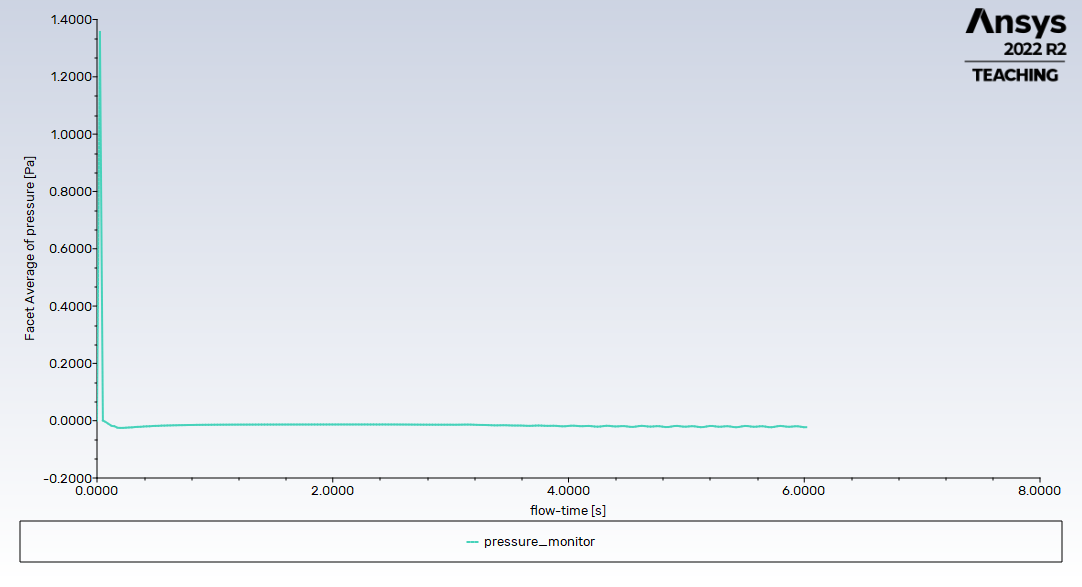
\includegraphics[width=0.8\textwidth]{Questions/Figures/pressure plot grid 3 2.png}
    \caption{Pressure at P1 over time for Grid 3-2}
    \label{fig:pressure plot grid 3 2}
\end{figure}
\begin{figure}[H]
    \centering
    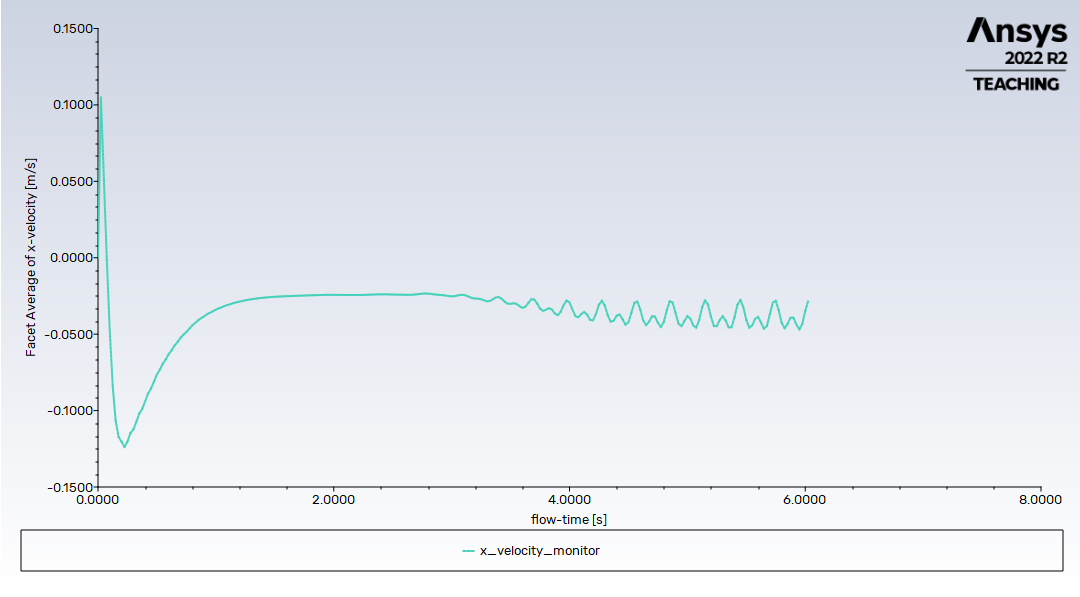
\includegraphics[width=0.8\textwidth]{Questions/Figures/x-velocity plot grid 3 2.png}
    \caption{Streamwise velocity at P1 over time for Grid 3-2}
    \label{fig:x-velocity plot grid 3 2}
\end{figure}
\begin{figure}[H]
    \centering
    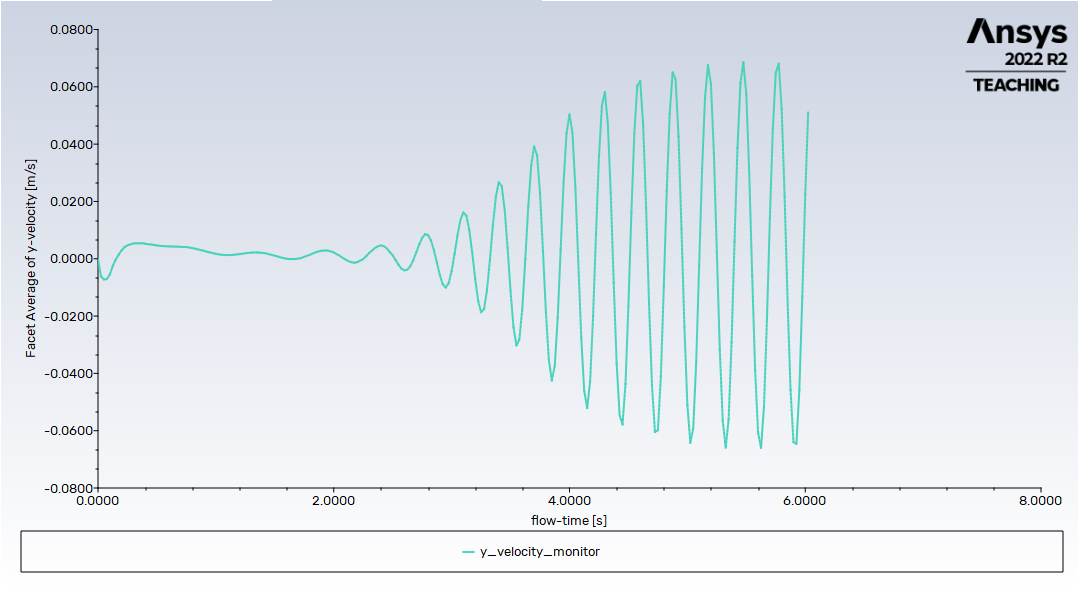
\includegraphics[width=0.8\textwidth]{Questions/Figures/y-velocity plot grid 3 2.png}
    \caption{Spanwise velocity at P1 over time for Grid 3-2}
    \label{fig:y-velocity plot grid 3 2}
\end{figure}

The period of vortex shedding is approximated from the y-velocity plot to be
\begin{align*}
    \tau &= 2(t_{\text{peak}} - t_{\text{trough}})
    &= 2(5.85 - 5.625)
    &= 0.45 \text{ s}
\end{align*}
The Strouhal number is then
\begin{align*}
    \text{St} &= \frac{fD}{U_\infty} \\
    &= \frac{1/0.45 \times 0.01}{0.20} \\ 
    &= \boxed{0.1111}
\end{align*}

The pressure and vorticity contours are shown in Figures \ref{fig:pressure contour grid 3 2} and \ref{fig:vorticity contour grid 3 2}.
\begin{figure}[H]
    \centering
    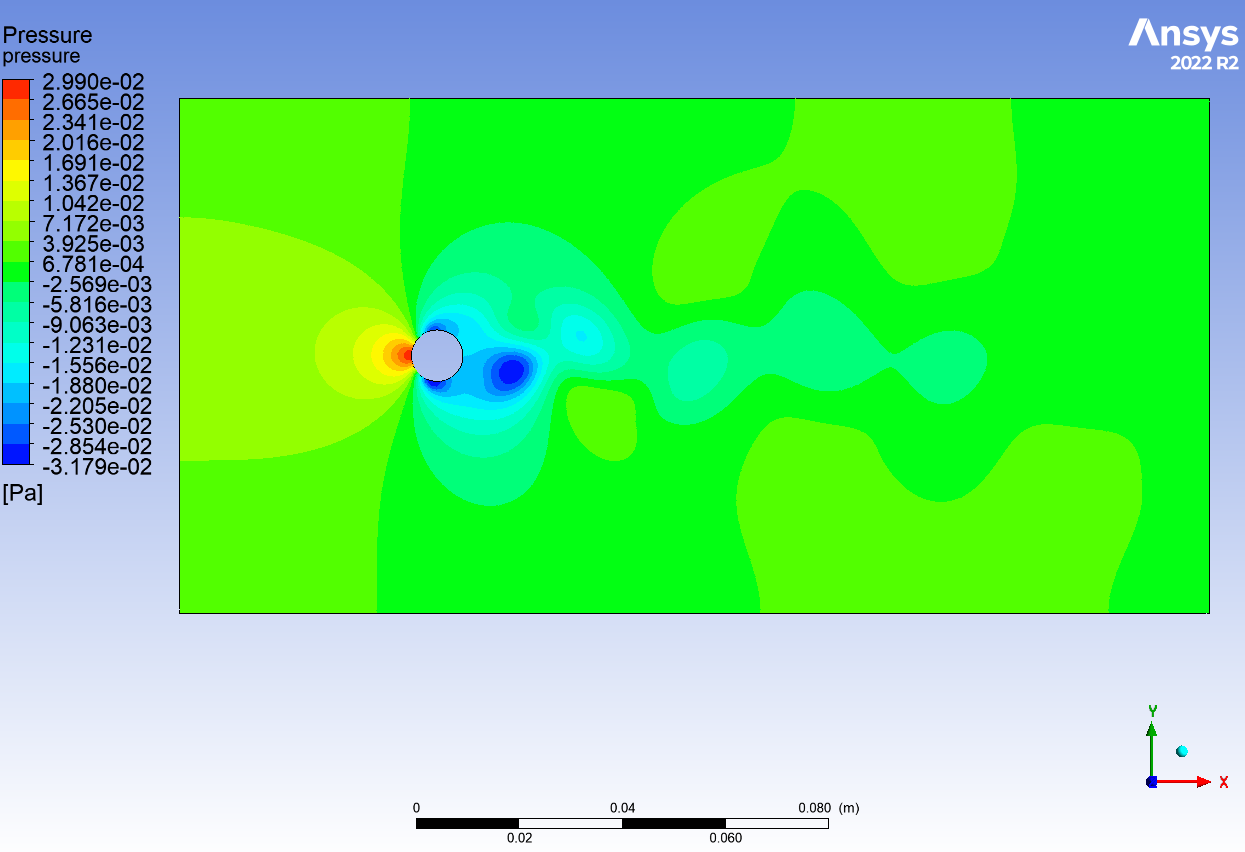
\includegraphics[width=0.8\textwidth]{Questions/Figures/pressure contour grid 3 2.png}
    \caption{Pressure Contour for Grid 3-2}
    \label{fig:pressure contour grid 3 2}
\end{figure}
\begin{figure}[H]
    \centering
    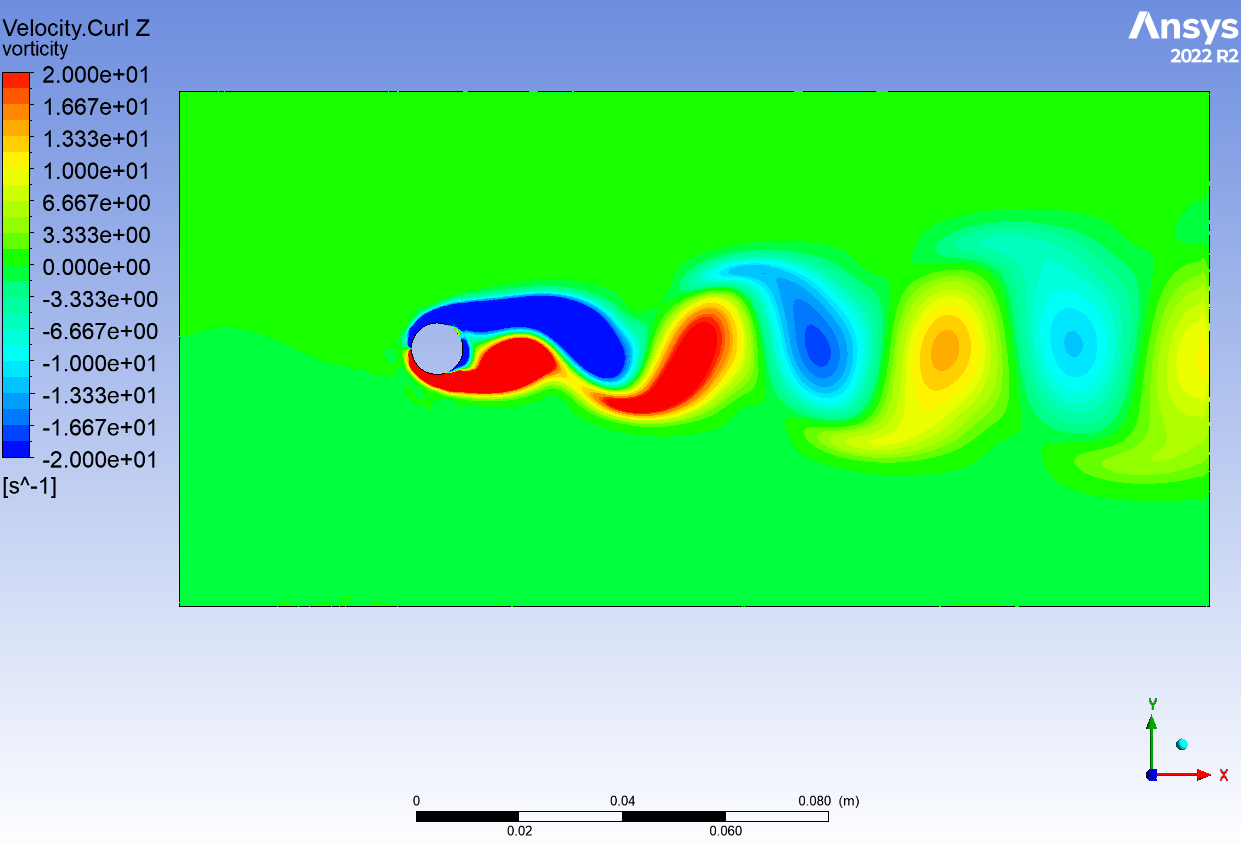
\includegraphics[width=0.8\textwidth]{Questions/Figures/vorticity contour grid 3 2.png}
    \caption{Vorticity Contour for Grid 3-2}
    \label{fig:vorticity contour grid 3 2}
\end{figure}

The mean streamwise velocity and mean pressure contours are shown in Figures \ref{fig:mean x velocity along wake center line grid 3 2} and \ref{fig:mean pressure velocity contour grid 3 2}.
\begin{figure}[H]
    \centering
    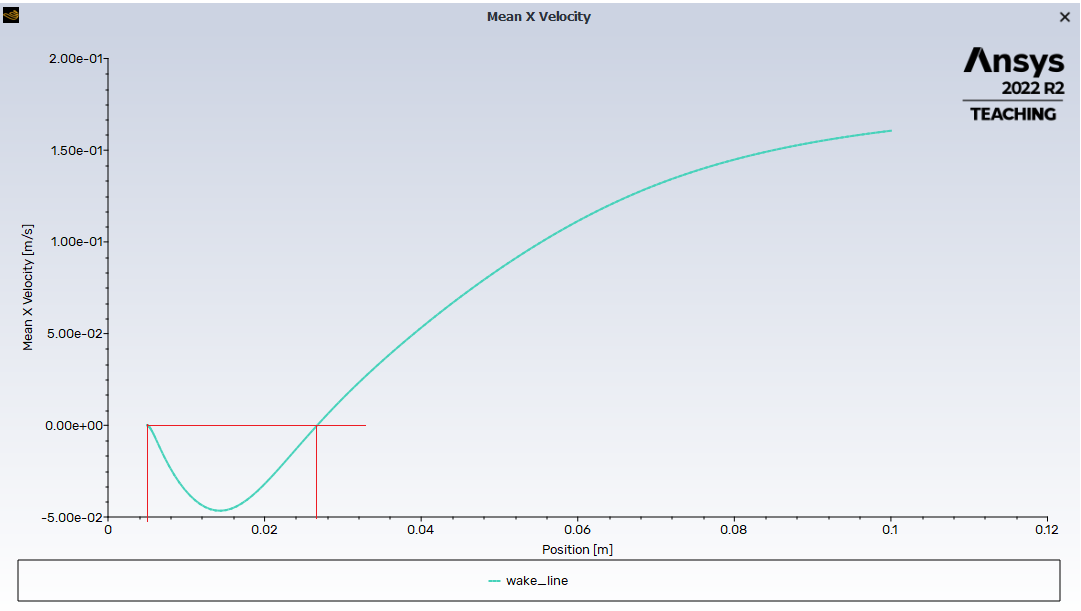
\includegraphics[width=0.8\textwidth]{Questions/Figures/mean x velocity along wake center line grid 3 2.png}
    \caption{Mean Streamwise Velocity for Grid 3-2}
    \label{fig:mean x velocity along wake center line grid 3 2}
\end{figure}
\begin{figure}[H]
    \centering
    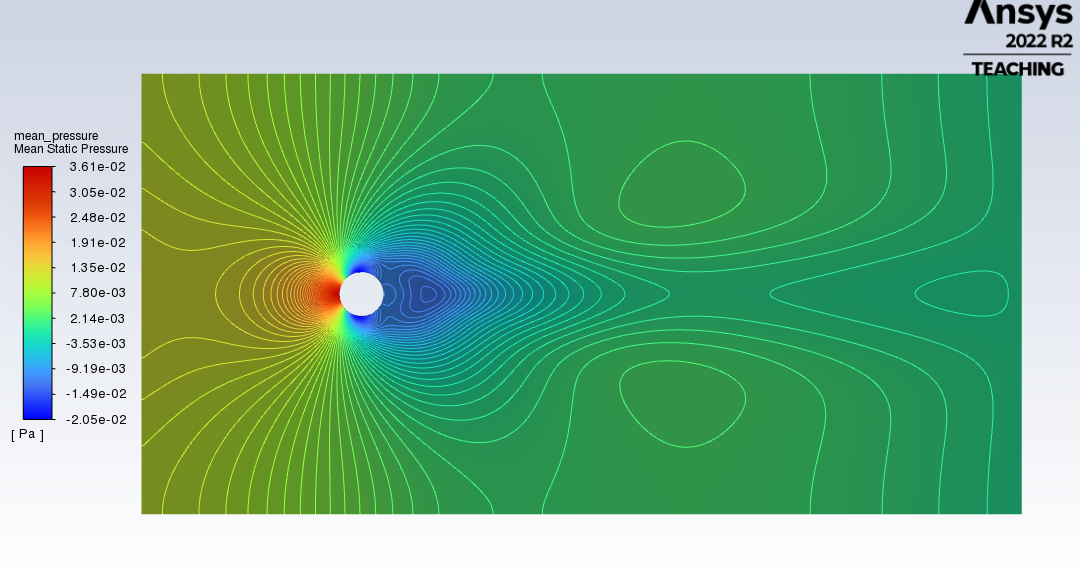
\includegraphics[width=0.8\textwidth]{Questions/Figures/mean pressure velocity contour grid 3 2.png}
    \caption{Mean Pressure Contour for Grid 3-2}
    \label{fig:mean pressure velocity contour grid 3 2}
\end{figure}
The recirculation length is approximately
\begin{align*}
    \hat{L}_r &= \frac{\Delta x}{D} \\
    &= \frac{0.026 - 0.005}{0.01} \\
    &= \boxed{2.1}
\end{align*}

\subsubsection{Grid 3-3}
The number of iterations has been updated to
\begin{align*}
    \text{Iterations} &= \frac{T_{\text{total}}}{\Delta t} \\
    &= \frac{10}{0.25} \\
    &= \boxed{40}
\end{align*}

\begin{figure}[H]
    \centering
    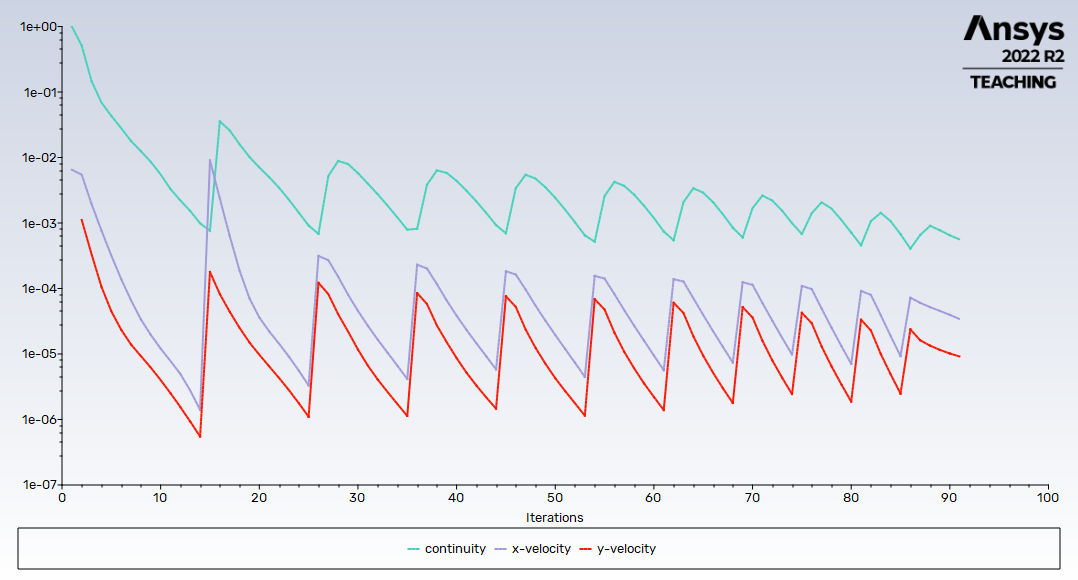
\includegraphics[width=0.8\textwidth]{Questions/Figures/residuals plot grid 3 3.png}
    \caption{Residuals for Grid 3-3}
\end{figure}

The mean and drag plots are shown in Figures \ref{fig:drag force plot grid 3 3} and \ref{fig:lift force plot grid 3 3}.
\begin{figure}[H]
    \centering
    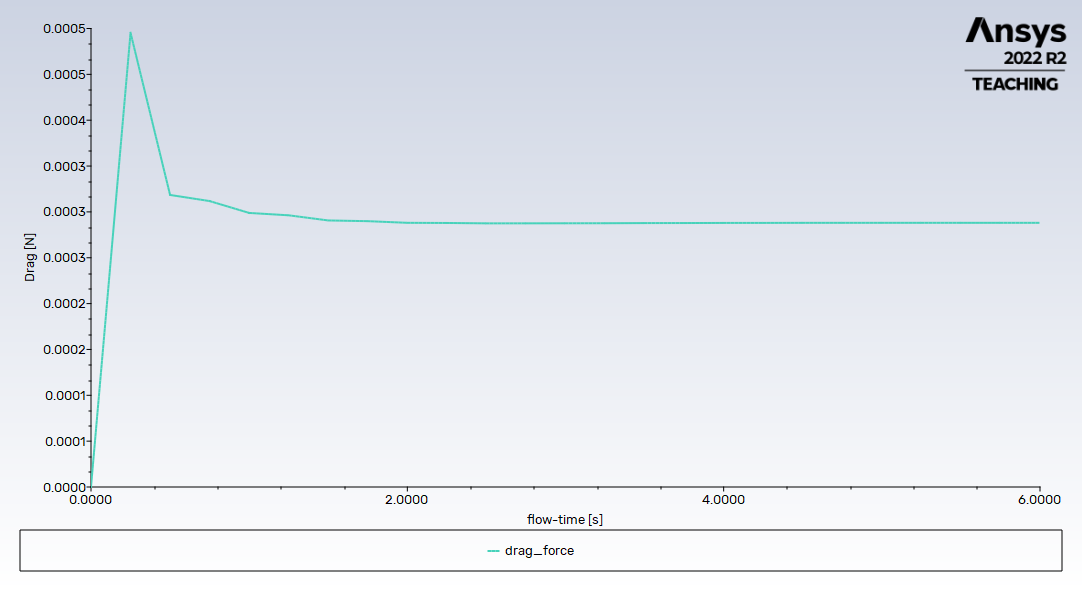
\includegraphics[width=0.8\textwidth]{Questions/Figures/drag force plot grid 3 3.png}
    \caption{Drag force over time for Grid 3-3}
    \label{fig:drag force plot grid 3 3}
\end{figure}
\begin{figure}[H]
    \centering
    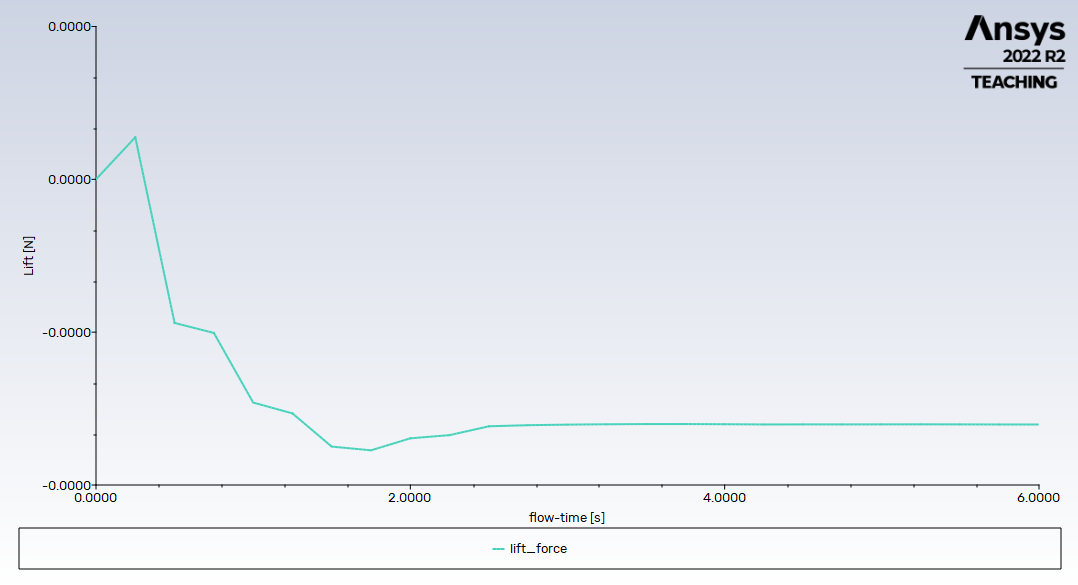
\includegraphics[width=0.8\textwidth]{Questions/Figures/lift force plot grid 3 3.png}
    \caption{Lift force over time for Grid 3-3}
    \label{fig:lift force plot grid 3 3}
\end{figure}
The mean drag force is
\begin{align*}
    F_D &= \frac{F_{D_{\text{max}}} + F_{D_{\text{min}}}}{2} \\
    &= \frac{2.88\times10^{-4} + 2.88\times10^{-4}}{2} \\
    &= \boxed{2.88\times10^{-4} \text{ N}}
\end{align*}
The mean lift force is
\begin{align*}
    F_L &= \frac{F_{L_{\text{max}}} + F_{L_{\text{min}}}}{2} \\
    &= \frac{-8.02\times10^{-7} - 8.02\times10^{-7}}{2} \\
    &= \boxed{-8.02\times10^{-7} \text{ N}}
\end{align*}
Then, the mean drag coefficient is
\begin{align*}
    C_d &= \frac{F_D}{0.5\rho U_\infty^2 D} \\
    &= \frac{2.88\times10^{-4}}{0.5 \times 1.184 \times 0.20^2 \times 0.01} \\
    &= \boxed{1.216}
\end{align*}
The mean lift coefficient is
\begin{align*}
    C_l &= \frac{F_L}{0.5\rho U_\infty^2 D} \\
    &= \frac{-8.02\times10^{-7}}{0.5 \times 1.184 \times 0.20^2 \times 0.01} \\
    &= \boxed{-3.39\times10^{-3}}
\end{align*}

The pressure and velocity plots are shown in Figures \ref{fig:pressure plot grid 3 3}, \ref{fig:x-velocity plot grid 3 3}, and \ref{fig:y-velocity plot grid 3 3}.
\begin{figure}[H]
    \centering
    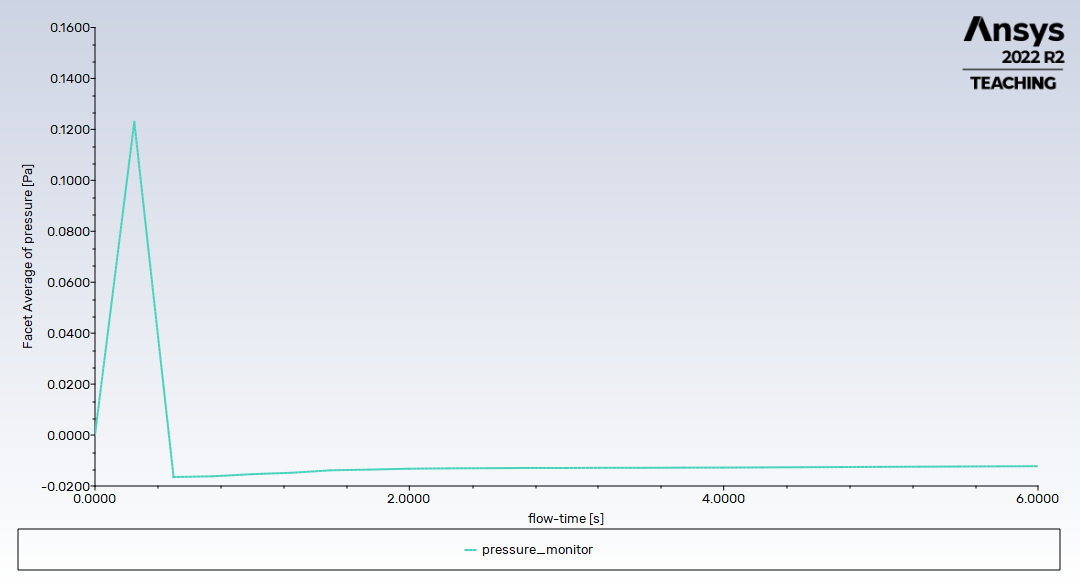
\includegraphics[width=0.8\textwidth]{Questions/Figures/pressure plot grid 3 3.png}
    \caption{Pressure at P1 over time for Grid 3-3}
    \label{fig:pressure plot grid 3 3}
\end{figure}
\begin{figure}[H]
    \centering
    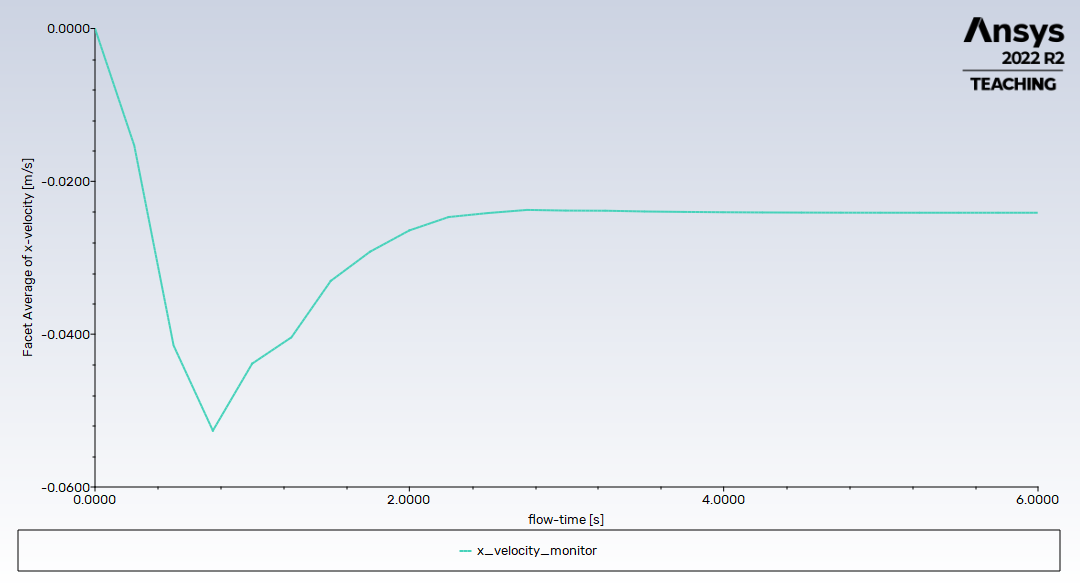
\includegraphics[width=0.8\textwidth]{Questions/Figures/x-velocity plot grid 3 3.png}
    \caption{Streamwise velocity at P1 over time for Grid 3-3}
    \label{fig:x-velocity plot grid 3 3}
\end{figure}
\begin{figure}[H]
    \centering
    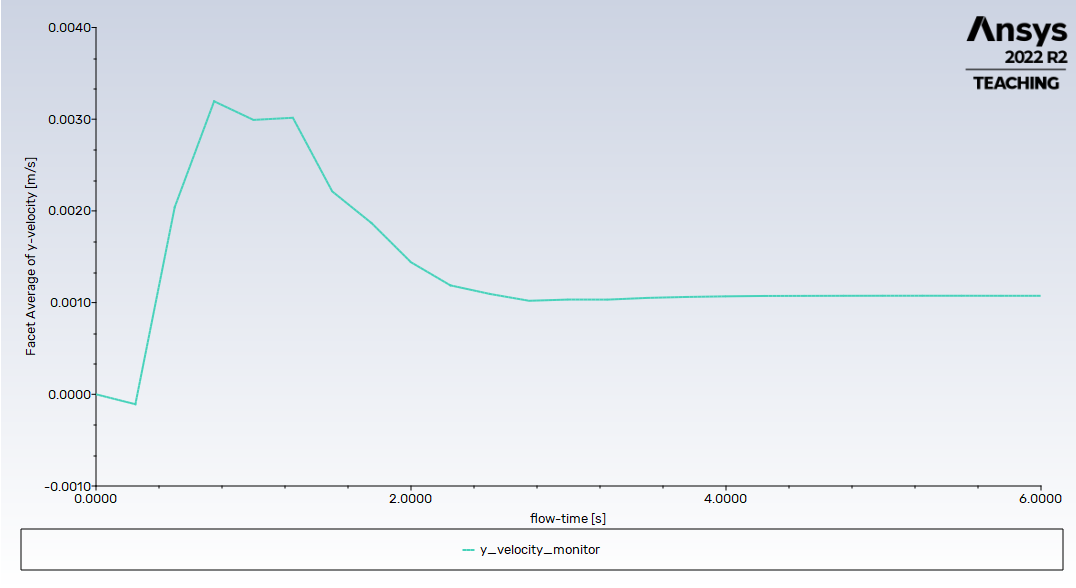
\includegraphics[width=0.8\textwidth]{Questions/Figures/y-velocity plot grid 3 3.png}
    \caption{Spanwise velocity at P1 over time for Grid 3-3}
    \label{fig:y-velocity plot grid 3 3}
\end{figure}

The period of vortex shedding in the y-velocity plot could not be determined due to the lack of a clear quasi-steady state region. Defining period as 2, the duration of the steady region, the Strouhal number is then
\begin{align*}
    \text{St} &= \frac{fD}{U_\infty} \\
    &= \frac{1/2 \times 0.01}{0.20} \\ 
    &= \boxed{0.025}
\end{align*}

The pressure and vorticity contours are shown in Figures \ref{fig:pressure contour grid 3 3} and \ref{fig:vorticity contour grid 3 3}.
\begin{figure}[H]
    \centering
    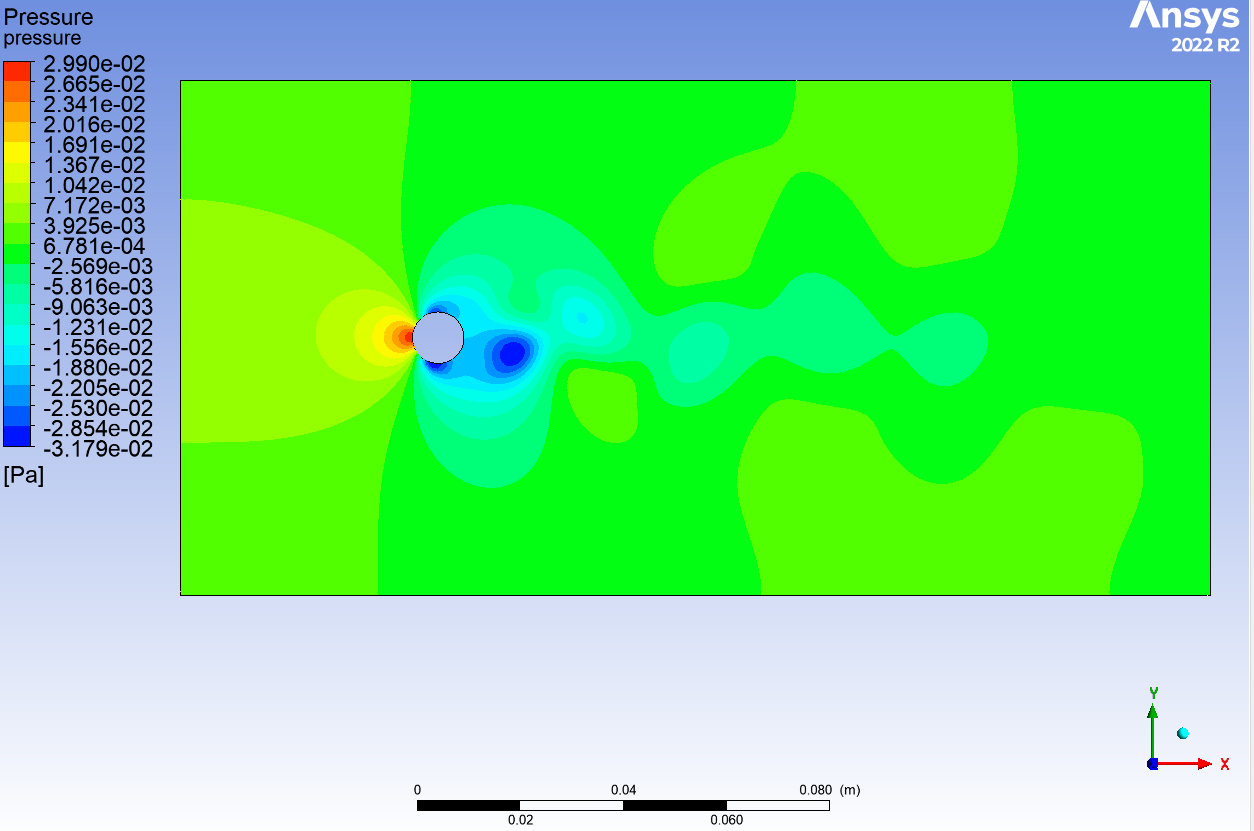
\includegraphics[width=0.8\textwidth]{Questions/Figures/pressure contour grid 3 3.png}
    \caption{Pressure Contour for Grid 3-3}
    \label{fig:pressure contour grid 3 3}
\end{figure}
\begin{figure}[H]
    \centering
    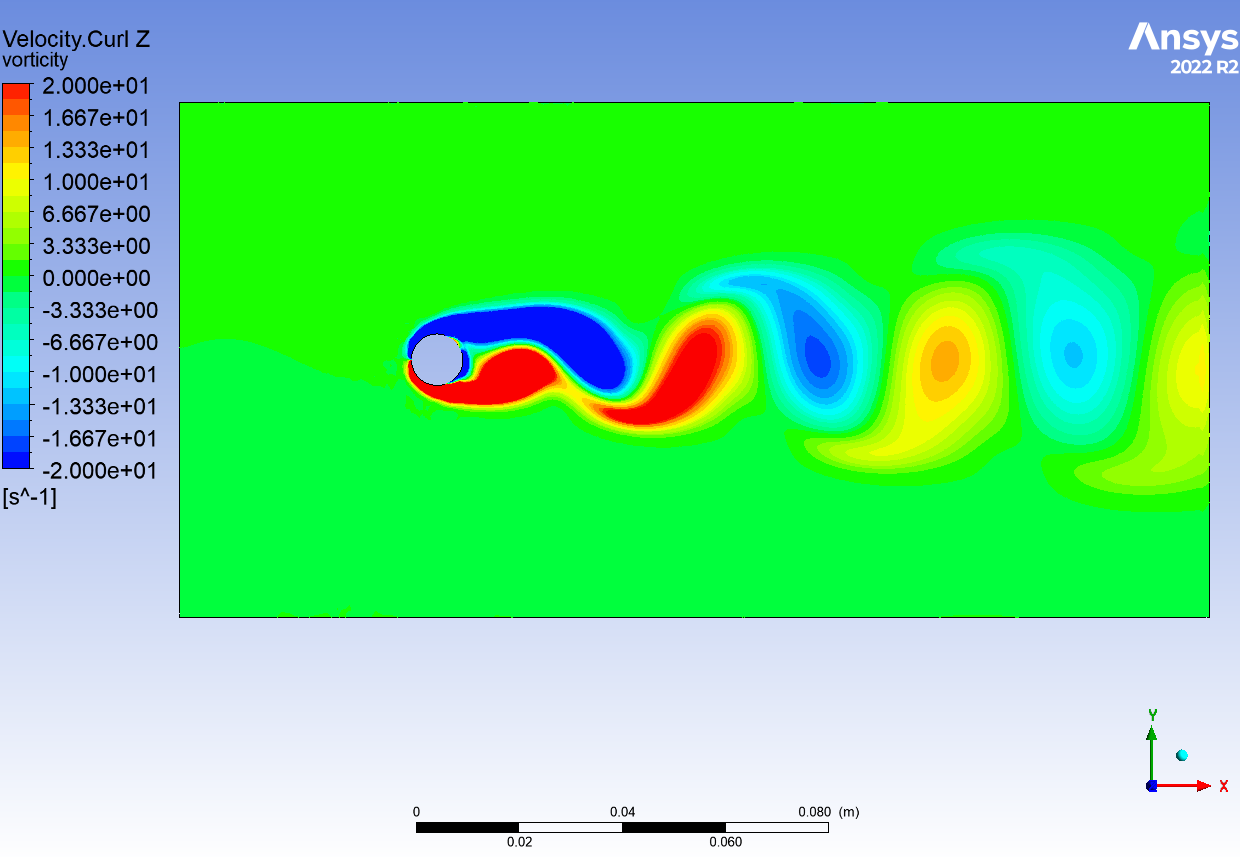
\includegraphics[width=0.8\textwidth]{Questions/Figures/vorticity contour grid 3 3.png}
    \caption{Vorticity Contour for Grid 3-3}
    \label{fig:vorticity contour grid 3 3}
\end{figure}

The mean streamwise velocity and mean pressure contours are shown in Figures \ref{fig:mean x velocity along wake center line grid 3 3} and \ref{fig:mean pressure velocity contour grid 3 3}.
\begin{figure}[H]
    \centering
    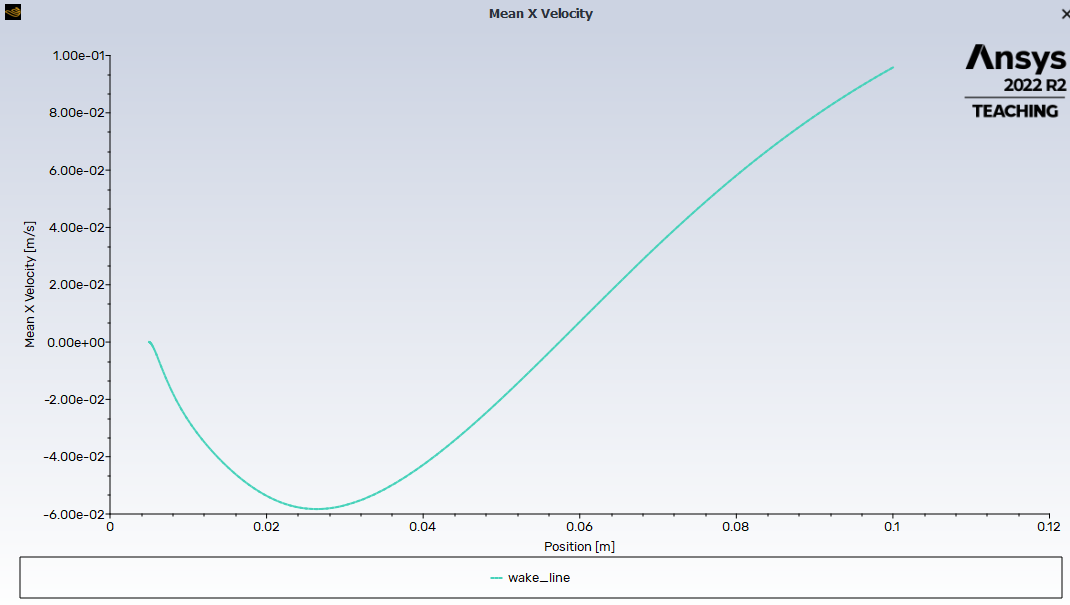
\includegraphics[width=0.8\textwidth]{Questions/Figures/mean x velocity along wake center line grid 3 3.png}
    \caption{Mean Streamwise Velocity for Grid 3-3}
    \label{fig:mean x velocity along wake center line grid 3 3}
\end{figure}
\begin{figure}[H]
    \centering
    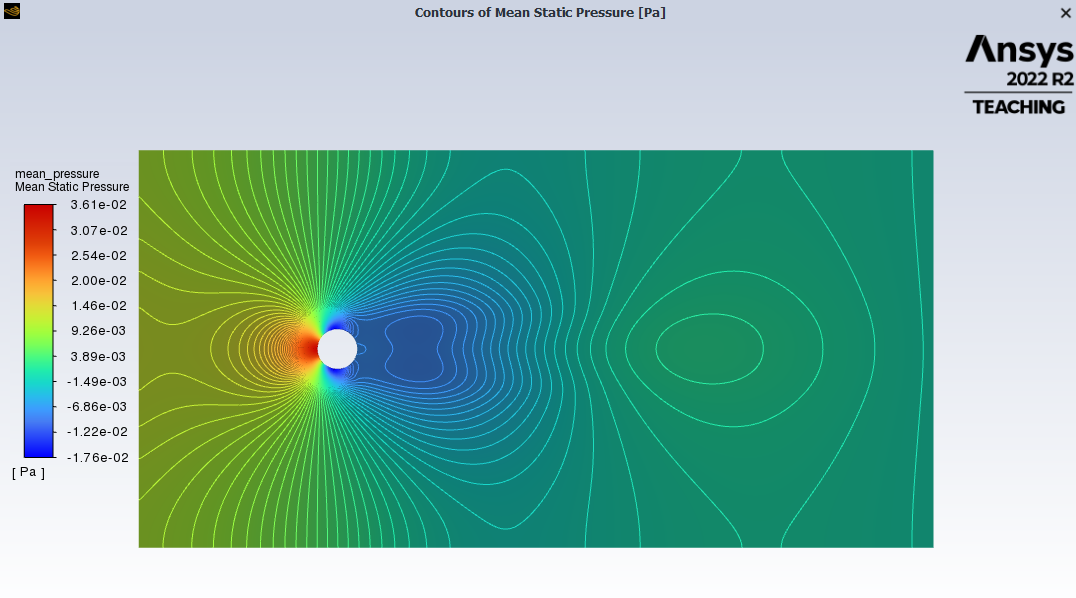
\includegraphics[width=0.8\textwidth]{Questions/Figures/mean pressure velocity contour grid 3 3.png}
    \caption{Mean Pressure Contour for Grid 3-3}
    \label{fig:mean pressure velocity contour grid 3 3}
\end{figure}
The recirculation length is approximately
\begin{align*}
    \hat{L}_r &= \frac{\Delta x}{D} \\
    &= \frac{0.057 - 0.005}{0.01} \\
    &= \boxed{5.2}
\end{align*}

\subsection{Task 3.2}
\textit{Create a table that shows the main wake parameters (Mean Recirculation Length, Mean Drag Coefficient, Mean Lift Coefficient, and St) you calculated for “Grid 3”, “Grid 3-2” and “Grid 3-3”. Include their percentage change with respect to those of “Grid 3”. Also, compare the contour plots of pressure and mean pressure for the three cases.}

The results are summarized in Table \ref{tab:summary of results}.
\begin{table}[H]
    \centering
    \caption{Summary of Results for Grids 3, 3-2, and 3-3}
    \label{tab:summary of results}
    \begin{tabular}{cccccccccc}
        \toprule
        Grid & $C_d$ & $C_l$ & $\hat{L}_r$ & St & $\Delta C_d \%$ & $\Delta C_l \%$ & $\Delta \hat{L}_r \%$ & $\Delta \text{St} \%$ \\
        \midrule
        3 & 1.512 & -0.00186 & 1.5 & 0.1887 & - & - & - & - \\
        3-2 & 1.444 & -0.00112 & 2.1 & 0.1111 & -4.497 & -39.785 & 40 & -40 \\
        3-3 & 1.216 & -0.00339 & 5.2 & 0.025 & -19.577 & 82.258 & 246.667 & -86.957 \\
        \bottomrule
    \end{tabular}
\end{table}
Refering to Figures \ref{fig:pressure contour grid 3}, \ref{fig:pressure contour grid 3 2} and \ref{fig:pressure contour grid 3 3}, the vortex shedding is most distinguishable in Grid 3. Some detail is lost in Grid 3-2, and the vortex shedding is not visible in Grid 3-3. In fact, the pressure contour for Grid 3-3 almost looks like a mean pressure contour.

Refering to Figures \ref{fig:mean pressure velocity contour grid 3}, \ref{fig:mean pressure velocity contour grid 3 2} and \ref{fig:mean pressure velocity contour grid 3 3}, the grids look very similar. The detail of the pressure contours have been smoothed out by taking the mean. 

\subsection{Task 3.3}
\textit{Comment on the differences between the three temporal grids. Which case should be appropriate for wake analysis? Why?}\\

For wake analysis, Grid 3 is deemed the most suitable option. Its smaller timestep effectively captures a greater level of detail in the unsteady flow characteristics. This is evident in the pressure and vorticity contours, which exhibit more detailed representations, particularly in displaying vortex shedding, compared to larger timesteps. Larger timesteps tend to emphasize the mean flow rather than the specific flow characteristics at a given location.

Of course, smaller timesteps will take longer to simulate. If time is a constraint, Grid 3-2 is a suitable compromise. It still captures the vortex shedding, but with less detail. Grid 3-3 is not suitable for wake analysis, as it does not capture the vortex shedding detail appropriately.



